% from ega4-2-fr.tex
\oldpage[IV-2]{199}

\begin{proof}
Considérons l'homomorphisme complété
$\widehat\varphi:\widehat A\to\widehat{A'}$ et le morphisme correspondant
$\widehat f={}^a\widehat\varphi$; on a le diagramme commutatif
\[
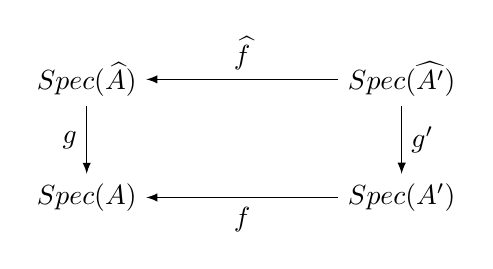
\begin{tikzpicture}[>=latex]
\node (tl) at (0,1.5) {$\operatorname{Spec}(\widehat A)$};
\node (tr) at (4,1.5) {$\operatorname{Spec}(\widehat{A'})$};
\node (bl) at (0,0) {$\operatorname{Spec}(A)$};
\node (br) at (4,0) {$\operatorname{Spec}(A')$};
\draw[->] (tr) -- node[above] {$\widehat f$} (tl);
\draw[->] (tl) -- node[left] {$g$} (bl);
\draw[->] (tr) -- node[right] {$g'$} (br);
\draw[->] (br) -- node[below] {$f$} (bl);
\end{tikzpicture}
\]
où $g$ et $g'$ sont les morphismes canoniques. Comme par hypothèse $f$ est
un $\boldsymbol P$-morphisme et $g'$ un morphisme régulier, il résulte de
$(\mathrm P_{\mathrm I})$ que $f\circ g'=g\circ\widehat f$ est un
$\boldsymbol P$-morphisme. D'autre part, l'hypothèse que $f$ est un
$\boldsymbol P$-morphisme implique que $f$ est plat, donc il en est de même
de $\widehat f$ (Bourbaki, \emph{Alg. comm.}, chap. III, \S~5,
n\textsuperscript{o}~4, cor. de la prop. 3), qui est d'ailleurs un
homomorphisme local, donc fidèlement plat (0$_{\mathrm I}$, 6.6.2); il
résulte alors de $(\mathrm P_{\mathrm{II}})$ que $g$ est un
$\boldsymbol P$-morphisme.
\end{proof}

\begin{corollary}[7.4.3]
\label{IV.2.s7.4.3-fr}
\begin{enumerate}
\item[\emph{(i)}] Soient $A$ un $\boldsymbol P$-anneau local noethérien,
$A'=\widehat A$ son complété. Supposons que pour tout idéal premier
$\mathfrak p'$ de $A'$, les fibres formelles de $A'_{\mathfrak p'}$ soient
géométriquement régulières; alors, pour tout idéal premier $\mathfrak p$ de
$A$, $A_{\mathfrak p}$ est un $\boldsymbol P$-anneau.
\item[\emph{(ii)}] Supposons que $\boldsymbol P$ vérifie la condition
$(\mathrm P_{\mathrm{IV}})$ (7.3.6). Soient $A$ un $\boldsymbol P$-anneau
local noethérien, $B$ une $A$-algèbre locale essentiellement de type fini,
et telle que l'homomorphisme $A\to B$ soit local. Posons $A'=\widehat A$,
et soit $\mathfrak n'$ l'unique idéal premier de
$B'=B\otimes_A A'$ au-dessus de l'idéal maximal de $B$ et de l'idéal
maximal de $A'$. Si les fibres formelles de $B'_{\mathfrak n'}$ sont
géométriquement régulières, alors $B$ est un $\boldsymbol P$-anneau.
\end{enumerate}
\end{corollary}

\begin{proof}
\begin{enumerate}
\item[\emph{(i)}] Comme par hypothèse
$\operatorname{Spec}(A')\to\operatorname{Spec}(A)$ est un
$\boldsymbol P$-morphisme, il en est de même de
$\operatorname{Spec}(A'_{\mathfrak p'})\to
\operatorname{Spec}(A_{\mathfrak p})$ en vertu de (7.3.2, b)), pour tout
idéal premier $\mathfrak p$ de $A$ et tout idéal premier $\mathfrak p'$ de
$A'$ au-dessus de $\mathfrak p$. Il suffit alors d'appliquer le lemme
(7.4.2) à ce morphisme, en remarquant que le morphisme
$\operatorname{Spec}(A')\to\operatorname{Spec}(A)$ est surjectif.
\item[\emph{(ii)}] En vertu de (7.4.2), il suffit de prouver que le morphisme
$\operatorname{Spec}(B'_{\mathfrak n'})\to\operatorname{Spec}(B)$ est un
$\boldsymbol P$-morphisme. Or on a $B=C_{\mathfrak n}$, où $C$ est une
$A$-algèbre de type fini et $\mathfrak n$ un idéal premier de $C$ au-dessus
de l'idéal maximal de $A$. Si on pose $C'=C\otimes_A A'$, il résulte des
hypothèses et de (7.3.7) que
$\operatorname{Spec}(C')\to\operatorname{Spec}(C)$ est un
$\boldsymbol P$-morphisme; comme $B'_{\mathfrak n'}$ est un anneau local en
un idéal premier de $C'$ au-dessus de $\mathfrak n$, la conclusion résulte
de (7.3.2, b)).
\end{enumerate}
\end{proof}

\begin{theorem}[7.4.4]
\label{IV.2.s7.4.4-fr}
Les hypothèses sur $\boldsymbol P$ étant celles de (7.4.1), soit $A$ un
$\boldsymbol P$-anneau local noethérien.
\begin{enumerate}
\item[\emph{(i)}] Pour tout idéal premier $\mathfrak p$ de $A$,
$A_{\mathfrak p}$ est un $\boldsymbol P$-anneau.
\item[\emph{(ii)}] Supposons en outre que $\boldsymbol P$ vérifie la condition
$(\mathrm P_{\mathrm{IV}})$. Alors tout anneau local qui est une
$A$-algèbre essentiellement de type fini est un $\boldsymbol P$-anneau.
\end{enumerate}
\end{theorem}

\begin{proof}
\begin{enumerate}
\item[\emph{(i)}] Appliquant (7.4.3, (ii)), tout revient à voir que pour tout
idéal premier $\mathfrak p'$ de $A'=\widehat A$,
$A'_{\mathfrak p'}$ a ses fibres formelles géométriquement régulières. Or,
cela a été démontré dans (0, 22.3.3 et 22.5.8).

